%
% libskry - Algorithms summary
%
% Filip Szczerek, 2019-10-20
%
% document tested with pdfTeX 3.14159265-2.6-1.40.19 (TeX Live 2018)
%

\documentclass[12pt]{article}
\usepackage[lighttt]{lmodern}
\usepackage[a4paper, margin=1in]{geometry}
\usepackage{amsmath}
\usepackage{float}
\usepackage{listings}
\usepackage{color}
\usepackage{graphicx}

\usepackage{hyperref}
\usepackage[all]{hypcap} % needed to help hyperlinks direct correctly

\hypersetup{
    colorlinks,
    citecolor=black,
    filecolor=black,
    linkcolor=black,
    urlcolor=black
}

\graphicspath{{images/}}

\ttfamily
\DeclareFontShape{OT1}{lmtt}{m}{it}{<->sub*lmtt/m/sl}{}

\definecolor{gray}{cmyk}{0,0,0,0.05}
\definecolor{darkgray}{cmyk}{0,0,0,0.85}
\definecolor{darkblue}{rgb}{0,0,0.65}
\definecolor{darkgreen}{rgb}{0,0.5,0}

\newcommand{\nbd}{\nobreakdash}

% \DeclareRobustCommand*{\ora}{\overrightarrow}

% ----------------------------------------------------------------------------------------------------------------------
\begin{document}

\title{libskry --- Lucky imaging implementation for the~Stackistry project
\ \\
\ \\
\emph{Algorithms summary}}
\author{Filip Szczerek}
\date{2019-10-20}
\maketitle

\tableofcontents

\lstset{
    basicstyle=\ttfamily\small,
    % commentstyle=\rmfamily\slshape\small,
    commentstyle=\color{darkgray},
    keywordstyle=\color{darkgreen}\bfseries,
    language=C,
    backgroundcolor=\color{gray},
    deletekeywords={int,unsigned,char,void,short,float,double,long},
    morekeywords={
        restrict
    },
    classoffset=1,
    morekeywords={
        int,unsigned,char,void,short,float,double,long,
        ptrdiff_t,
        uint8_t,
        uint64_t,
        size_t,
    },
    keywordstyle=\color{darkblue},
    classoffset=0
}

\newpage

% ----------------------------------------------------------------------------------------------------------------------
\section{Overview}

This~document describes the~algorithms used by \emph{libskry}\footnote{\url{https://github.com/GreatAttractor/libskry}},
an~image stacking implementation for the~\emph{Stackistry}\footnote{\url{https://github.com/GreatAttractor/Stackistry}}
project.

Source code relevant for the~discussed feature is shown in listing boxes:

\begin{lstlisting}
size_t SKRY_get_img_count(const SKRY_ImgSequence *img_seq);
\end{lstlisting}

% ----------------------------------------------------------------------------------------------------------------------
\section{Input and output}

The~input to \emph{libskry} is an~\emph{image sequence} (i.e. a~video). The primary output is an~\emph{image stack} --
a~single image built from the~video, with an~improved signal-to-noise ratio and deformations removed.

Additional outputs are the~\emph{best fragments composite} -- consisting of best-quality fragments of all images;
and image quality data for the~whole sequence.

% ----------------------------------------------------------------------------------------------------------------------
\section{Internal pixel formats}

All processing phases except the~final image stacking (shift\nbd-and\nbd-add summation) operate on
8\nbd-bit grayscale images. In the~last phase, image stacking uses the~same number of channels as the~input
video and produces an~image stack with 32\nbd-bit floating\nbd-point channel values.

Raw\nbd-color images are demosaiced (debayered) using simple bilinear interpolation for all processing phases except
image stacking, which uses high-quality linear interpolation\footnote{Rico Malvar, Li-wei He, Ross Cutler
\emph{High\nbd-Quality Linear Interpolation for Demosaicing of Bayer-Patterned Color Images}; International Conference
of Acoustic, Speech and Signal Processing, May 2004.
\url{https://www.microsoft.com/en-us/research/publication/high-quality-linear-interpolation-for-demosaicing-of-bayer-patterned-color-images/}}.

\begin{lstlisting}[caption={Demosaicing functions ({\ttfamily{demosaic.h/.c}})}]
enum SKRY_demosaic_method
void demosaic_8_as_RGB(...);
void demosaic_8_as_mono8(...);
void demosaic_16_as_RGB(...);
void demosaic_16_as_mono8(...);
enum SKRY_CFA_pattern translate_CFA_pattern(...);
\end{lstlisting}

% ----------------------------------------------------------------------------------------------------------------------
\section{Image quality}\label{sec:quality}

\emph{Image quality} is defined for images (and image fragments) as the~sum of absolute differences between pixel values
of the~image and its blurred version:

\[
quality = \sum | I - I_{blur} |
\]

In other words, it is the~sum of pixel values of the image's high\nbd-frequency component. Higher values correspond to
better quality.

Image blurring is performed with a~box filter applied three times, which gives results quite close to Gaussian blur and
has short running time.

\lstset{emph={detail_scale},emphstyle=\bfseries}
\begin{lstlisting}[caption={Image quality ({\ttfamily{filters.h/.c, quality.h/.c}})}. Box blur radius is specified as the parameter {\ttfamily{detail\_scale}}.]
#define QUALITY_ESTIMATE_BOX_BLUR_ITERATIONS 3

SKRY_QualityEstimation* SKRY_init_quality_est(
    const SKRY_ImgAlignment* img_algn,
    unsigned estimation_area_size,
    /// Corresponds to box blur radius
    /// used for quality estimation.
    unsigned detail_scale
);

SKRY_quality_t estimate_quality(...);

struct SKRY_image* box_blur_img(...);
\end{lstlisting}
\lstset{emph={}}

% ----------------------------------------------------------------------------------------------------------------------
\section{Block matching}\label{sec:blockmatching}

Block matching is used during the~image alignment and reference point alignment phases.

Given the~position of a~certain feature in an~image, the~aim is to find the~position of the~same feature in another
image(s). It is done by comparing the~feature's \emph{reference block} (an~image fragment around the~feature's position)
with other images, around the~currently known position.

The~reference block is overlayed onto the~new image, at search positions surrounding the~feature's last known position
within a~certain radius and spacing (\emph{search step}). The~initial search step is $>1$, and is halved after each
search iteration.

A~search iteration involves calculating the~sum of squared pixel value differences of the~underlying image fragment and
the~reference block. The~position with the~smallest sum becomes the~initial search position for the~next iteration.

After the~first iteration, the~search radius equals the~search step of the~previous iteration. Once the~search step
reaches 1, the~best position becomes the~feature's new position.

\begin{lstlisting}[caption={Block matching ({\ttfamily{match.h/.c}})}]
uint64_t calc_sum_of_squared_diffs(...);
void find_matching_position(...);
\end{lstlisting}

% ----------------------------------------------------------------------------------------------------------------------
\section{Processing phases}

% ----------------------------------------------------------------------------------------------------------------------
\subsection{Image alignment (video stabilization)}\label{sec:imgalignment}

Image alignment compensates any global image drift/shaking etc. Two modes are available: anchors and image centroid.

Anchor-based alignment performs block\nbd-matching around user- or automatically\nbd-selec\-ted anchor point(s).
Automatic selection puts an~anchor in the~highest\nbd-quality fragment in the~inner area of the~first image of the~input
sequence.

Centroid\nbd-based alignment simply uses the~image centroid as the~reference position. It is best suited for planetary
videos.

\begin{lstlisting}[caption={Image alignment ({\ttfamily{img\_align.h/.c}})}]
enum SKRY_img_alignment_method {...};
SKRY_ImgAlignment* SKRY_init_img_alignment(...);
enum SKRY_result SKRY_img_alignment_step(...);
\end{lstlisting}

Regardless of the~mode used, the~result of image alignment is a~list of offsets, one for each image in the~sequence.
The~offsets taken together define an~intersection of all images, which is the~region visible in the~whole video.

\begin{lstlisting}
struct SKRY_img_alignment
{
    // ...

    /// Set-theoretic intersection of all images after alignment
    /// (i.e. the fragment which is visible in all images).
    struct
    {
        /// Offset, relative to the first image's origin.
        struct SKRY_point offset;

        /// Coordinates of the bottom right corner
        /// (belongs to the intersection), relative
        /// to the first image's origin.
        struct SKRY_point bottom_right;

        unsigned width;
        unsigned height;
    } intersection;

    struct SKRY_point* img_offsets;
};
\end{lstlisting}

This "region of interest" (referred to as \emph{images' intersection} throughout the~code) is what the~subsequent
processing phases operate on.

% ----------------------------------------------------------------------------------------------------------------------
\subsection{Quality estimation}\label{sec:quality_estimation}

The~goal of quality estimation is selecting image fragments for use by subsequent processing phases. The~method of
calculating the~quality is given in \ref{sec:quality}.

The~images' intersection (\ref{sec:imgalignment}) is divided into square \emph{quality estimation areas} (plus any
residual rectangles along the~right and bottom border).

\begin{figure}[H]
\centering
\includegraphics{quality_estimation_areas.pdf}
\caption{Quality estimation areas.}
\end{figure}

Each area's quality is calculated for each image in the~sequence. After quality estimation completes, individual areas
and whole images can be sorted by quality; additionally, a~composite image containing the~best image fragments
(corresponding to quality estimation areas) of the~whole sequence can be assembled (figs. \ref{fig:qualitysun},
\ref{fig:quality_moon}).

For each estimation area, its \emph{reference block} is stored, which is the~image fragment underlying this area and its
neighboring (3x3) areas, taken from the~image where the~area has the~best quality (fig. \ref{fig:quality_ref_block}).

\begin{figure}[H]
\centering
\includegraphics{qual_area_ref_block.pdf}
\caption{Quality estimation area and its reference block.}
\label{fig:quality_ref_block}
\end{figure}

\begin{figure}[H]
\centering
\includegraphics[width=0.8\textwidth]{quality_sun.png}
\caption{Results of quality estimation of a~1377-frame 60-second video of the~Sun in white light (aperture: 180 mm). Top
to bottom: the~best image, the~worst image, composite of best image fragments -- note that in the~composite,
the~granulation is visible everywhere. Estimation area size: 40x40 pixels.}
\label{fig:qualitysun}
\end{figure}

\begin{figure}[H]
\centering
\includegraphics[width=0.62\textwidth]{quality_moon.png}
\caption{Results of quality estimation of a~500-frame 17-second video of the~Moon (aperture: 300 mm). Top to bottom:
the~best image, the~worst image, composite of best image fragments. Estimation area size: 40x40 pixels.}
\label{fig:quality_moon}
\end{figure}

\begin{figure}[H]
\centering
\includegraphics[width=1.1\textwidth]{seeing_comparison.pdf}
\caption[caption]{Comparison of the~frame quality and the~output of a~\emph{Solar Scintillation Seeing Monitor} for
a~50-second 20-fps video of the~Sun in H$\alpha$. % FIXME: should be typeset with upright alpha: Hα
The~quality has been mapped to the~range $[0, 1]$, where 0 = best, 1 = worst. Better (lower) seeing values in arc
seconds generally correspond to better frame quality. Note, however, that an image deformed without blurring does not
decrease the~quality value, but may correspond to a~stronger momentary scintillation.

EJ Seykora \emph{Solar scintillation and the~monitoring of solar seeing}\\
\url{http://adsabs.harvard.edu/full/1993SoPh..145..389S}.}
\end{figure}

% ----------------------------------------------------------------------------------------------------------------------
\subsection{Reference point alignment}

Apart from inducing blurring, atmospheric seeing also distorts the~images. These deformations have to be compensated for
during final image stacking.

The~distortion is tracked by placing a~number of reference points within the~images' intersection
(\ref{sec:imgalignment}) and tracing their positions throughout the~image sequence via block matching
(\ref{sec:blockmatching}). Each reference point has an associated \emph{reference block} (of user-specified size) copied
from the~underlying quality estimation area's reference block (fig. \ref{fig:quality_ref_block}); i.e. it contains
the~best-quality fragment of the~whole image sequence at this position.

\begin{lstlisting}[caption={Reference point alignment ({\ttfamily{ref\_pt\_align.h/.c}})}]
SKRY_RefPtAlignment *SKRY_init_ref_pt_alignment(
    const SKRY_QualityEstimation *qual_est,
    /// Number of elements in 'points'; if zero, points will be
    /// placed automatically.
    size_t num_points,
    /// Reference point positions; if null, points will be
    /// placed automatically.
    /** Positions are specified within the images' intersection.
        The points must not lie outside it. */
    const struct SKRY_point *points,

    /// Criterion for updating ref. point position
    /// (and later for stacking).
    enum SKRY_quality_criterion quality_criterion,
    /// Interpreted according to 'quality_criterion'.
    unsigned quality_threshold,

    /// Size (in pixels) of reference blocks used for
    /// block matching.
    unsigned ref_block_size,

    /// Search radius (in pixels) used during block matching.
    unsigned search_radius,

    /// If not null, receives operation result.
    enum SKRY_result *result,

    // Parameters used if num_points==0 (automatic placement
    // of ref. points) -------------------------------------

    /// Min. image brightness that a ref. point can be placed at
    /// (values: [0; 1]).
    /** Value is relative to the image's darkest (0.0)
        and brightest (1.0) pixels. Used only during automatic
        placement. */
    float placement_brightness_threshold,

    /// Structure detection threshold; value of 1.2
    /// is recommended.
    /** The greater the value, the more local contrast
        is required to place a ref. point. */
    float structure_threshold,

    /** Corresponds to pixel size of smallest structures.
        Should equal 1 for optimally-sampled or undersampled
        images. Use higher values for oversampled (blurry)
        material. */
    unsigned structure_scale,

    /// Spacing in pixels between reference points.
    unsigned spacing
);
\end{lstlisting}

% ----------------------------------------------------------------------------------------------------------------------
\subsubsection{Initialization}

The~user may place the~reference points themselves, or choose automatic placement. In case of the~latter, the~following
parameters control the~placement:

\begin{itemize}
\item \emph{spacing}
\nopagebreak

Defines the~step of a~square grid; in each grid cell at most one reference point is placed. An additional search
for the~best position within a~grid cell is performed (see the~function \lstinline$SKRY_suggest_ref_point_positions()$
in {\ttfamily quality.c}).

\item \emph{brightness threshold}
\nopagebreak

A~value from $[0, 1]$, where 0 corresponds to the~darkest and 1 to the~brightest pixel of all quality estimation areas'
reference blocks (fig. \ref{fig:quality_ref_block}). A~reference point can only be placed at a~position whose brightness
in the~corresponding quality estimation area's ref.~block is $>=$ threshold.

\item \emph{structure threshold \& scale}
\nopagebreak

Determine how much structure (high-contrast features) must be present at a~location to place a~reference point. Since
the~points will be tracked using block matching, this is assessed by checking the~sum of squared differences of pixel
values of the~image fragment surrounding the~reference point and image fragments in two concentric shells around it
(fig. \ref{fig:ref_point_assess}) --- higher sum is desirable. See~\lstinline$assess_ref_pt_location()$ in
{\ttfamily quality.c}.

\end{itemize}

\begin{figure}[H]
\centering
\includegraphics{ref_point_assessment.pdf}
\caption{Assessment of the~block-matching eligibility of a~prospective reference point position. The~reference block is
compared to image fragments at surrounding locations in two concentric shells (gray dots). The~higher the~sums of
squared differences of pixel values, the~better the~position (\lstinline$assess_ref_pt_location()$).}
\label{fig:ref_point_assess}
\end{figure}

An additional criterion for judging a~reference point position is the~distribution of gradient directions around it.
If the~histogram of gradient directions is insufficiently filled, the~position is rejected. For instance, if the~image
is locally dominated by a~single edge (e.g. the~limb of overexposed solar disc, without prominences or resolved
spicules), should block matching be performed, the~tracked point would jump along the~edge. See the~function
\lstinline$assess_gradients_for_block_matching()$ in {\ttfamily misc.c}.

% ----------------------------------------------------------------------------------------------------------------------
\subsubsection{Quality criteria}\label{sec:quality_criteria}

Finding of new positions of reference points in an image is performed only when the~underlying quality estimation area
has (in this image) quality that meets the~user-specified criterion (see the~enumeration
\lstinline$SKRY_quality_criterion$). It can be one of the~following:

\begin{itemize}
\item \emph{Percentage of best-quality fragments}
\nopagebreak

Only use the~specified \% of the best\nbd-quality fragments.

\item \emph{Minimum relative quality percentage}
\nopagebreak

Only use the~fragments with quality above the~specified threshold: \% relative to $[min, max]$ of the~corresponding
quality estimation area.

\item \emph{Number of best-quality fragments}

Only use the~specified number of best fragment.

\end{itemize}

% ----------------------------------------------------------------------------------------------------------------------
\subsubsection{Triangulation and point tracking}\label{sec:triangulation}

The~final processing phase, image stacking (\ref{sec:stacking}), operates on triangular patches of the~region of
interest (\ref{sec:imgalignment}). The~triangles are created as follows (fig. \ref{fig:triangulation}):

\begin{itemize}
\item a~number of additional fixed reference points are added outsite the~region of interest, along its edges
\item three fixed reference points are added, creating a~triangle enveloping all the~other points
\item a~Delaunay triangulation of the~whole point set is determined
\end{itemize}

\begin{figure}[H]
\centering
\includegraphics{triangulation.pdf}
\caption{Triangulation of reference points. Black dots: regular (tracked) points, red dots: fixed points.
(see \lstinline$append_fixed_point()$).}
\label{fig:triangulation}
\end{figure}

Once the~triangulation is known, for each input image, for each triangle, the~new positions of its vertices (except for
the~fixed points) are found by block matching (\ref{sec:blockmatching}) iff the~current sum of qualities of their
underlying quality estimation areas meets the~user\nbd-specified criterion (\ref{sec:quality_criteria}). (A~check is
performed not to update a~vertex more than once.)

This process produces a~list of valid positions of each reference point (\lstinline{ref_pt_align.c}):

\begin{lstlisting}
struct reference_point
{
    //...

    struct
    {
        struct SKRY_point pos;
        int is_valid; ///< True if the quality criteria
                      /// for the image are met.
    } *positions; ///< Array of positions in every active image.
};
\end{lstlisting}

The~per-image positions are then averaged to provide the~final/undistorted position of each point
(\lstinline{SKRY_get_final_positions()}), later used for stacking. The~averaging is important for making time\nbd-lapse
animations (i.e. sequences of stacks made of a~number of input videos); otherwise, if a~randomly distorted reference
point position were taken as the~"true" position, each stack would have a~slightly different geometry and the~whole
time lapse would be "wobbly" (showing deformations frame\nbd-to\nbd-frame).

% ----------------------------------------------------------------------------------------------------------------------
\subsection{Image stacking}\label{sec:stacking}

Image stacking is the shift-and-add summation of high-quality (\ref{sec:quality_criteria}) fragments, eventually
producing a~\emph{stack} with improved signal\nbd-to\nbd-noise ratio and input video deformations removed.

\subsubsection{Initialization}

\begin{lstlisting}[caption={Stacking initialization ({\ttfamily{stacking.h/.c}})}]
SKRY_Stacking *SKRY_init_stacking(
    const SKRY_RefPtAlignment *ref_pt_align,

    /// May be null; no longer used after the function returns.
    const SKRY_Image *flatfield,

    /// If not null, receives operation result.
    enum SKRY_result *result
);
\end{lstlisting}

Stacking operates on the~triangular patches (\ref{sec:triangulation}) which cover the~region of interest
(\ref{sec:imgalignment}). Each triangle is rasterized --- a~list of its pixels is created, together with their
barycentric coordinates (fig. \ref{fig:rasterization}); the~averaged point positions are~used here.
\footnote{The~triangulation was determined for the~initial reference point positions; with the~averaged positions,
the~Delaunay condition may be no longer met. This is of no consequence for stacking.}

\begin{figure}
\centering
\includegraphics{rasterization.pdf}
\caption{Left: rasterization of triangular patches (see \lstinline$rasterize\_triangle()$). Right:~triangle's pixels
(black, white and red dots). Barycentric coordinates of the~pixel marked with red dot are $u=\frac{2}{11},
v=\frac{6}{11}$ (corresponding to $\vec{CA}$, $\vec{CB}$).}
\label{fig:rasterization}
\end{figure}

Then the~stacking buffer (accumulator) is allocated; for each pixel of the~region of interest, it contains
an~accumulated pixel value (single\nobreakdash-precision floating\nobreakdash-point value per channel) and a~counter
which stores the~number of source pixels used to calculate the~accumulated value.

% ----------------------------------------------------------------------------------------------------------------------
\subsubsection{Summation}

The shift\nbd-and\nbd-add summation proceeds as follows:

\begin{list}{$\bullet$}{}
    \item For each input image:
    \begin{list}{$\bullet$}{}
        \item For each triangle, if the~quality criterion is met (\ref{sec:quality_criteria}):
        \begin{list}{$\bullet$}{}
            \item For each pixel from the triangle's rasterization list (fig.~\ref{fig:rasterization}):
            \begin{list}{$\bullet$}{}
                \item Use the barycentric coordinates to find the~(deformed) pixel coordinates in the~input image,
                      perform bilinear interpolation of pixel values in the~input image, add the~interpolated value to
                      the~stacking accumulator.
            \end{list}
        \end{list}
    \end{list}
\end{list}

In addition, if the~user has specified a~\emph{flat-field}\footnote{An~image, preferably captured by pointing
the~optical system at a~uniformly lit background, which shows illumination non\nbd-uniformity caused by the~optical
train, e.g.~vignetting, etalon "sweet\nbd-spot", etc.}, the~source value is corrected by the~local flat\nbd-field value
(taking the~image alignment offset (\ref{sec:imgalignment}) into account). The whole process is illustrated in detail in
figs.~\ref{fig:stacking1}, \ref{fig:stacking2}.

Finally, the~complete stack is produced by dividing each accumulated pixel value by its corresponding counter. (Also, at
each step of the~stacking phase, a~partial stack can be generated the same way.)

\begin{figure}
\centering
\includegraphics{stacking.pdf}
\caption{Left: triangle in the stacking accumulator, with one of its pixels marked. Right: the~same location in
the~deformed triangles in input images.}
\label{fig:stacking1}
\end{figure}

\begin{figure}
\centering
\includegraphics{stacking2.pdf}
\caption{For each pixel of the stacked triangle $\triangle ABC$ (red dot), its position in input image is obtained by
mapping barycentric coordinates $u, v$ from $\triangle ABC$ to the~deformed $\triangle A'B'C'$. After bilinear
interpolation of the~closest neighbors (white dots), the~value is added to the~stacking accumulator.}
\label{fig:stacking2}
\end{figure}


% ----------------------------------------------------------------------------------------------------------------------
\section{Post-processing}

An~image stack (\ref{sec:stacking}) is typically fuzzy (unless the~input video was captured in perfect seeing
conditions) and requires post\nbd-processing, which usually includes sharpening and tone mapping
(fig.~\ref{fig:postproc}). The~latter especially benefits from using a~stacked image, which has a~much improved
signal\nbd-to\nbd-noise ratio; for instance, the~darker areas can be "stretched" quite liberally before image noise
becomes visible.

\begin{figure}
\centering
\includegraphics[width=1.0\textwidth]{postproc.png}
\caption{Top: image stack (Sun in H$\alpha$, aperture: 90 mm). Bottom: image stack with Lucy--Richardson deconvolution and unsharp masking applied in
\emph{ImPPG} (\url{https://greatattractor.github.io/imppg/}).}
\label{fig:postproc}
\end{figure}



\end{document}
